% lualatex presentation

\documentclass[svgnames]{beamer}
\usepackage[utf8]{inputenc}
\usepackage{fontspec}
\usepackage{arev}
\usepackage{beramono}
\usepackage{fontawesome}
\usepackage{manfnt}
\usepackage{xcolor}
\usepackage{listings}
\usepackage{hyperref}

\usetheme{default}
\setbeamertemplate{navigation symbols}
{%
%  \hspace{3em}
%  \vbox{%
%  \hbox{\insertslidenavigationsymbol}
%  \hbox{\insertframenavigationsymbol}
%  \hbox{\insertbackfindforwardnavigationsymbol}
%  \vspace{2em}}
}

\setbeamercolor{alerted text}{fg=red!70!black}
\setbeamercolor{structure}{fg=Navy}
\definecolor{wrong}{rgb}{0.7, 0, 0}
\definecolor{right}{rgb}{0, 0.5, 0}
\definecolor{gitred}{rgb}{0.6, 0, 0}
\definecolor{gitgreen}{rgb}{0, 0.5, 0}
\definecolor{gitbrown}{rgb}{0.6, 0.3, 0}


\hypersetup{%
  pdftitle={Introduction to Version Control with Git}
  ,pdfauthor={Gert-Ludwig Ingold <gert.ingold@physik.uni-augsburg.de>}
  ,pdfsubject={Tutorial at EuroSciPy 2017, Erlangen 29.8.2017}
  ,pdfkeywords={Git, version control system, tutorial, EuroSciPy}
}

\lstset{%
  language={}
  ,basicstyle={\ttfamily\scriptsize}
  ,alsoletter=$
  ,backgroundcolor=\color{black!10}
}

\graphicspath{{./images/}}

\begin{document}

\begin{frame}

 \vspace{1truecm}
 \begin{center}
  \structure{\large\textbf{Introduction to Version Control with Git}}\\[0.3truecm]
  \structure{Gert-Ludwig Ingold}

  \vspace{1.5truecm}
  \faicon{github}\ \ttfamily{\scriptsize https://github.com/gertingold/euroscipy-git-tutorial.git}
 \end{center}
\end{frame}

\begin{frame}
 \begin{center}
  \uncover<1->{\bfseries Do you write 100\% bugfree code with all features implemented from the very
	       beginning?\\[0.1truecm]
	       \normalfont yes: 0 points / no: 1 point}

  \vspace{0.2truecm}
  \uncover<2->{\textbullet}

  \vspace{0.2truecm}
  \uncover<2->{\bfseries Do you collaborate with others?\\[0.1truecm]
	       \normalfont yes: 1 point / no: 0 points}

  \vspace{0.2truecm}
  \uncover<3->{\textbullet}

  \vspace{0.2truecm}
  \uncover<3->{\bfseries Do you want to contribute to open software?\\[0.1truecm]
	       \normalfont yes: 1 point / no: 0 points}

  \vspace{0.8truecm}
  \uncover<4>{\alert{\bfseries One or more points: Version control is for you!}}
 \end{center}

\end{frame}

\begin{frame}{A short history of version control}
 \begin{itemize}
  \item \textit{SCCS -- Source Code Control System (1972)}
  \item \textit{RCS -- Revision Control System (1982)}\\
	single file oriented, locking mechanism
  \item \textit{CVS -- Concurrent Versions System (1990)}\\
	\textit{Subversion (2000)}\\
	centralized version control system
  \item \textit{\alert<2>{Git}, Mercurial, Bazaar (2005)}\\
	distributed version control systems
 \end{itemize}

 \begin{center}
  \uncover<2>{
\includegraphics[width=\textwidth]{git_def}}
 \end{center}
\end{frame}

\begin{frame}{Centralized version control systems}
 \begin{center}
  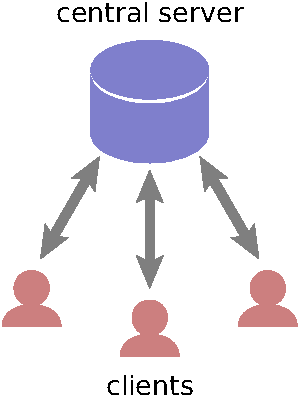
\includegraphics[width=\textwidth]{cvcs}
 \end{center}

 At any time, the central server contains well defined revisions
 of file sets which can be consecutively numbered.
\end{frame}

\begin{frame}{Distributed version control systems}
 \begin{center}
  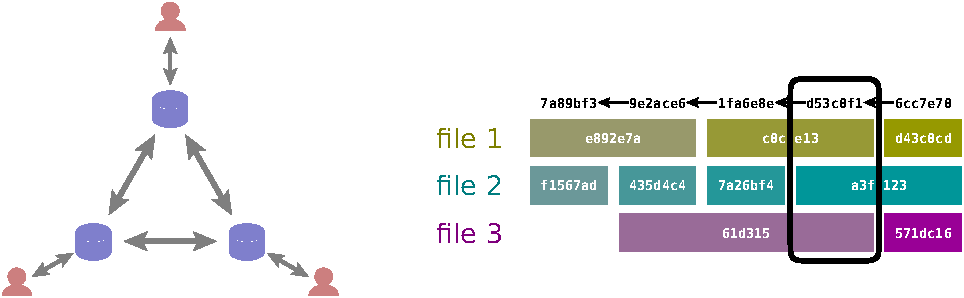
\includegraphics[width=\textwidth]{dvcs}
 \end{center}

 \begin{itemize}
  \item each individual repository has its own history
  \item each object is identified by a SHA1 hash consisting of
	40 hexadecimal values
  \item there are more than $10^{48}$ different SHA1 hashes
  \item often the first seven hex digits are sufficient for identification
 \end{itemize}
\end{frame}

\begin{frame}{Distributed VCS with Gitlab / Github}
 \begin{center}
  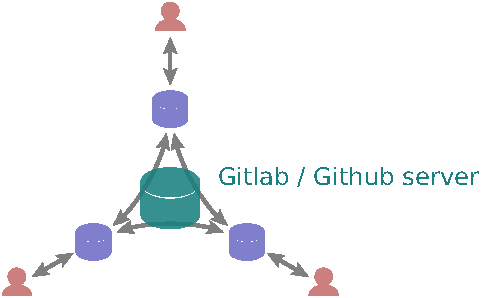
\includegraphics[height=0.6\textheight]{dvcs-github}
 \end{center}
\end{frame}

\begin{frame}{The prime time project}
 \textit{\structure{Question}}

 How many prime numbers can be interpreted as time in the format HH:MM?

 \vspace{1\baselineskip}
 \textit{\structure{Examples}}

 \textcolor{wrong}{2179 is a prime, but 21:79 is not a valid time}\\
 \textcolor{right}{2137 is a prime and 21:37 is a valid time}\\
 \textcolor{right}{953 is a prime and 9:53 is a valid time}\\
 \textcolor{wrong}{89 is a prime, but 0:89 is not a valid time}\\
 \textcolor{right}{41 is a prime and 0:41 is a valid time}\\
 \textcolor{right}{7 is a prime and 0:07 is a valid time}

 \vspace{1.5\baselineskip}
 \begin{center}
 \uncover<2>{\structure{\bfseries And, of course, we are going to use\\ a Git repository.}}
 \end{center}
\end{frame}

\begin{frame}[fragile]{Creating a respository}
 \structure{Initializing a new repository}

 \begin{lstlisting}
~/primetime$ git init
 \end{lstlisting}

 \vspace{\baselineskip}
 \structure{What has happened?}
 \begin{lstlisting}
~/primetime$ ls -a
.  ..  .git
~/primetime$ ls .git
branches  description  hooks  objects
config    HEAD         info   refs
 \end{lstlisting}

 \begin{center}
  \uncover<2>{\alert{\raisebox{0.5em}{\dbend}\quad Keep your hands off the \texttt{.git} directory!!!}}
 \end{center}
\end{frame}

\begin{frame}[fragile]{Tell Git who you are}

 \structure{Specify your name and your email address}
 \begin{lstlisting}
$ git config --global user.name <your name>
$ git config --global user.email <your email>
 \end{lstlisting}

 \vspace{\baselineskip}
 \structure{\ldots and, if you want, your preferred editor}
 \begin{lstlisting}
$ git config --global core.editor <editor>
 \end{lstlisting}

 \vspace{\baselineskip}
 \structure{example configuration}
 \begin{lstlisting}
$ git config --list
user.email=gert.ingold@physik.uni-augsburg.de
user.name=Gert-Ludwig Ingold
core.editor=vim
...
 \end{lstlisting}
\end{frame}

\begin{frame}[fragile]{It's prime time now}
 \texttt{primetime.py}
 \begin{lstlisting}
def istime(n):
    hh, mm = divmod(n, 100)
    return 0 <= hh <= 23 and 0 <= mm <= 59

print(sum(istime(n) for n in range(2360)))
 \end{lstlisting}

 \vspace{0.2truecm}
 \structure{What is the status?}
 \begin{lstlisting}[breaklines=true
                    ,escapechar=\%]
$git status
On branch master

Initial commit

Untracked files:
  (use "git add <file>..." to include in what will be committed)

        %\textcolor{gitred}{primetime.py}%

nothing added to commit but untracked files present (use "git add" to track)
 \end{lstlisting}
 \begin{itemize}
  \item Git has noticed our new file but ignores it
  \item Git tells us how to put the file under version control
 \end{itemize}
\end{frame}

\begin{frame}[fragile]{Adding a file}
 \begin{lstlisting}
~/primetime$ git add primetime.py
 \end{lstlisting}

 \vspace{0.2truecm}
 \structure{How did the status change?}
 \begin{lstlisting}[escapechar=\%]
~/primetime$ git status
On branch master

Initial commit

Changes to be committed:
  (use "git rm --cached <file>..." to unstage)

        %\textcolor{gitgreen}{new file:}%   %\textcolor{gitgreen}{primetime.py}%
 \end{lstlisting}
 \begin{itemize}
  \item Our file is now in the staging area, \alert{it is not under version control yet!}
  \item Our file can now be committed, but we can add more files first
  \item Git tells us how we can remove the file from the staging area if we put
        it there by accident
 \end{itemize}
\end{frame}

\begin{frame}{The way into the repository}
 \begin{center}
  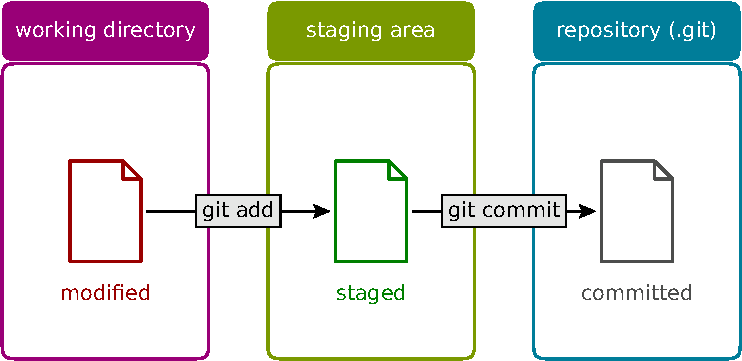
\includegraphics[width=0.9\textwidth]{addcommit}
 \end{center}
 \begin{itemize}
  \item All files present in the staging area are committed
  \item At a given time, different versions of a specific file can exist in
	any of the three areas
 \end{itemize}
\end{frame}

\begin{frame}[fragile]{Committing a file}
 \begin{lstlisting}
~/primetime$ git commit -m'added function to identify times'
[master (root-commit) 3733ef5] added function to identify times
 1 file changed, 5 insertions(+)
 create mode 100644 primetime.py
 \end{lstlisting}
 \begin{itemize}
  \item The option \texttt{-m} allows to specify a commit message
  \item Without this option, an editor is opened
  \item Limit the commit message to 50 characters
 \end{itemize}

 \vspace{0.2truecm}
 \structure{Check status to make sure that everything is fine}
 \begin{lstlisting}
~/primetime$ git status
On branch master
nothing to commit, working tree clean
 \end{lstlisting}
\end{frame}

\begin{frame}{Some tips on committing}
 \begin{itemize}
  \item A commit can contain several files, but all changes should
	represent a logical unit
  \item \textit{atomic commit:} Each commit refers only to a single
	basic change
  \item In most cases it is not a good idea to commit only at the
	end of a long working day
  \item If you have made unrelated changes but want to do an atomic
	commit, take a look at\\ \texttt{git add -p}
 \end{itemize}
\end{frame}

\begin{frame}[fragile]{A first complete version of primetime}
 \texttt{primes.py} (very inefficient)
 \begin{lstlisting}
def isprime(n):
    if n < 2: return False
    for divisor in range(2, n):
        if not n % divisor:
            return False
    return True
 \end{lstlisting}

 \vspace{0.2truecm}
 \texttt{primetime.py}
 \begin{lstlisting}
from primes import isprime

def istime(n):
    hh, mm = divmod(n, 100)
    return 0 <= hh <= 23 and 0 <= mm <= 59

print(sum(isprime(n) for n in range(2360) if istime(n)))
 \end{lstlisting}

 \vspace{0.4truecm}
 \structure{It works:}
 \begin{lstlisting}
~/primetime$ python primetime.py
211 
 \end{lstlisting}
\end{frame}

\begin{frame}[fragile]{The new status}
 \addtolength\linewidth{0.5truecm}
 \begin{lstlisting}[breaklines=true, escapechar=\%]
~/primetime$ git status
On branch master
Changes not staged for commit:
  (use "git add <file>..." to update what will be committed)
  (use "git checkout -- <file>..." to discard changes in working directory)

        modified:   %\textcolor{gitred}{primetime.py}%

Untracked files:
  (use "git add <file>..." to include in what will be committed)

        %\textcolor{gitred}{\_\_pycache\_\_/}%
        %\textcolor{gitred}{primes.py}%

no changes added to commit (use "git add" and/or "git commit -a")
 \end{lstlisting}
 \begin{itemize}
  \item Git noticed that \texttt{primetime.py} has been modified
  \item \texttt{primes.py} is new and not yet tracked by Git
  \item The directory \texttt{\_\_pycache\_\_/} should not be under version control
  \item Note also the help given by Git
 \end{itemize}
\end{frame}

\begin{frame}[fragile]{The \texttt{.gitignore} file}
 \begin{itemize}
  \item List in \texttt{.gitignore} line-by-line all directories and files to
	be ignored by Git
  \item * can be used as a wildcard
  \item Everything after a \# is a comment
  \item Put \texttt{.gitignore} under version control
  \item \texttt{.gitignore} can help to make sure that passwords never are put
	under version control
 \end{itemize}

 \vspace{0.3truecm}
 In our example:\\
 \texttt{.gitignore}
 \begin{lstlisting}
__pycache__/
 \end{lstlisting}
\end{frame}

\begin{frame}[fragile]{Add and commit}
 \begin{lstlisting}
~/primetime$ git add .gitignore
~/primetime$ git commit -m'.gitignore added'
[master c552c10] .gitignore added
 1 file changed, 1 insertion(+)
 create mode 100644 .gitignore
 \end{lstlisting}
 \begin{lstlisting}[escapechar=\%]
~/primetime$ git add primetime.py
~/primetime$ git add primes.py
~/primetime$ git status
On branch master
Changes to be committed:
  (use "git reset HEAD <file>..." to unstage)

        new file:   %\textcolor{gitgreen}{primes.py}%
        modified:   %\textcolor{gitgreen}{primetime.py}%

~/primetime$ git commit -m'first version of primetime completed'
[master 116fd26] first version of primetime completed
 2 files changed, 9 insertions(+), 1 deletion(-)
 create mode 100644 primes.py
 \end{lstlisting}
\end{frame}

\begin{frame}[fragile]{Branches}
 \begin{lstlisting}
~/primetime$ git status
On branch master
nothing to commit, working tree clean
 \end{lstlisting}
 \begin{itemize}
  \item We are on branch \texttt{master}, the default branch
 \end{itemize}
 \begin{lstlisting}[escapechar=\%]
gert@gli7440:~/primetime$ git branch
* %\textcolor{gitgreen}{master}%
 \end{lstlisting}
 \structure{What are branches good for?}
 \begin{itemize}
  \item Branches allow development of features without polluting
        the master branch
  \item Tip: Use a separate branch for each feature
  \item Unsuccessful experiments can easily be removed by deleting
        a branch
  \item In collaborative work, a pull request (see later) can easily
        focus on the new code
  \item Code can be merged into other branches
 \end{itemize}
\end{frame}

\begin{frame}[fragile]{Adding a new branch}
 In our prime time project, we are unhappy with our code for prime tests.
 Instead, we want to create a list of primes by means of the sieve of
 Eratosthenes. We develop the new feature in a separate branch so that the
 version in the master branch is always working.

 \begin{lstlisting}[breaklines=true]
~/primetime$ git checkout eratosthenes
error: pathspec 'eratosthenes' did not match any file(s) known to git.
 \end{lstlisting}
 \begin{itemize}
  \item \texttt{git checkout} changes between branches, but our branch
        does not yet exist. Use option \texttt{-b}
 \end{itemize}
 \begin{lstlisting}
gert@gli7440:~/primetime$ git checkout -b eratosthenes
Switched to a new branch 'eratosthenes'
 \end{lstlisting}

 \vspace{0.2truecm}
 Let us verify the branch
 \begin{lstlisting}[escapechar=\%]
gert@gli7440:~/primetime$ git branch
* %\textcolor{gitgreen}{eratosthenes}%
  master
 \end{lstlisting}
\end{frame}

\begin{frame}[fragile]{Improved primetime code (I)}
 \texttt{primes.py}
 \begin{lstlisting}
from math import sqrt
import numpy as np

def isprime(n):
    if n < 2: return False
    for divisor in range(2, n):
        if not n % divisor:
            return False
    return True

def eratosthenes(nmax):
    sieve = np.ones(nmax+1, dtype=np.bool)
    sieve[:2] = False
    for candidate in range(2, int(sqrt(nmax))+1):
        if sieve[candidate]:
            sieve[candidate*candidate::candidate] = False
    primes = np.arange(nmax+1)[sieve]
    return primes
 \end{lstlisting}
 \begin{lstlisting}
~/primetime$ git commit -a -m'added sieve of Eratosthenes'
[eratosthenes 982ae11] added sieve of Eratosthenes
 1 file changed, 12 insertions(+)
 \end{lstlisting}
\end{frame}

\begin{frame}[fragile]{Improved primetime code (II)}
 \addtolength\linewidth{0.7truecm}
 \texttt{primetime.py}
 \begin{lstlisting}
from primes import eratosthenes

def istime(n):
    hh, mm = divmod(n, 100)
    return 0 <= hh <= 23 and 0 <= mm <= 59

print(sum(istime(n) for n in eratosthenes(2359)))
 \end{lstlisting}
 \begin{lstlisting}
~/primetime$ git commit -a -m'make use of Eratosthenes in primetime'
[eratosthenes c9dfe03] make use of Eratosthenes in primetime
 1 file changed, 2 insertions(+), 2 deletions(-)
 \end{lstlisting}
\end{frame}

\begin{frame}[fragile]{Working on branches in parallel}
 In the meantime, an idea comes up to improve the function \texttt{isprime}.
 We make the corresponding changes in the master branch.

 First switch to the master branch:
 \begin{lstlisting}
~/primetime$ git checkout master
Switched to branch 'master'
 \end{lstlisting}

 Here, \texttt{primes.py} does not contain the function \texttt{eratosthenes}.
 We replace the code by
 \begin{lstlisting}
from math import sqrt

def isprime(n):
    if n < 2: return False
    for divisor in range(2, int(sqrt(n))+1):
        if not n % divisor:
            return False
    return True
 \end{lstlisting}
 \begin{lstlisting}
~/primetime$ git commit -a -m'improved prime test'
[master ebc424d] improved prime test
 1 file changed, 3 insertions(+), 1 deletion(-)
 \end{lstlisting}
\end{frame}

\begin{frame}[fragile]{Commits in different branches}
 \addtolength\linewidth{0.5truecm}
 \begin{lstlisting}[escapechar=\%]
~/primetime$ git log  --graph --branches --oneline
* %\textcolor{gitbrown}{ebc424d}% improved prime test
%\textcolor{gitred}{|}% * %\textcolor{gitbrown}{c9dfe03}% make use of Eratosthenes in primetime
%\textcolor{gitred}{|}% * %\textcolor{gitbrown}{982ae11}% added sieve of Eratosthenes
%\textcolor{gitred}{|/}%  
* %\textcolor{gitbrown}{116fd26}% first version of primetime completed
* %\textcolor{gitbrown}{c552c10}% .gitignore added
* %\textcolor{gitbrown}{3733ef5}% added function to identify times
 \end{lstlisting}

 \vspace{0.2truecm}
 \structure{Merging the content of the \texttt{eratosthenes} branch into the \texttt{master}
            branch}
 \begin{lstlisting}[escapechar=\%]
~/primetime$ git branch
  eratosthenes
  * %\textcolor{gitgreen}{master}%
  ~/primetime$ git merge eratosthenes
  Auto-merging primes.py
  CONFLICT (content): Merge conflict in primes.py
  Automatic merge failed; fix conflicts and then commit the result.
 \end{lstlisting}
 \begin{itemize}
  \item \texttt{primetime.py} corresponds now to the \texttt{eratosthenes} branch
  \item In \texttt{primes.py} a merge conflict needs to be resolved
 \end{itemize}
\end{frame}

\begin{frame}[fragile]{A merge conflict}
 \begin{lstlisting}[escapeinside=`´]
from math import sqrt
`\textcolor{red}{<\/<\/<\/<\/<\/<\/< HEAD}´
`\textcolor{red}{=======}´
`\textcolor{red}{import numpy as np}´
`\textcolor{red}{>\/>\/>\/>\/>\/>\/> eratosthenes}´

def isprime(n):
    if n < 2: return False
    for divisor in range(2, int(sqrt(n))+1):
        if not n % divisor:
            return False
    return True

def eratosthenes(nmax):
...
 \end{lstlisting}
 \begin{itemize}
  \item Alternative 1 between \texttt{>\/>\/>\/>\/>\/>\/>} and \texttt{=======}\\
	\texttt{HEAD} = version being merged into

  \item Alternative 2 between \texttt{=======} and \texttt{<\/<\/<\/<\/<\/<\/<}\\
	\texttt{eratosthenes} = version being merged
  \item Bring the file into the desired form and commit it
 \end{itemize}
\end{frame}

\begin{frame}[fragile]{Resolving a merge conflict}
 new version of \texttt{primes.py}
 \begin{lstlisting}
from math import sqrt
import numpy as np

def isprime(n):
    if n < 2: return False
...
 \end{lstlisting}
 \begin{lstlisting}
~/primetime$ git commit -a
[master 5782233] Merge branch 'eratosthenes'
 \end{lstlisting}
 \begin{lstlisting}[escapechar=\%]
~/primetime$ git log --graph --branches --oneline
*   %\textcolor{gitbrown}{5782233}% Merge branch 'eratosthenes'
%\textcolor{gitred}{|}\textcolor{gitgreen}{\textbackslash}%  
%\textcolor{gitred}{|}% * %\textcolor{gitbrown}{c9dfe03}% make use of Eratosthenes in primetime
%\textcolor{gitred}{| }%* %\textcolor{gitbrown}{982ae11}% added sieve of Eratosthenes
* %\textcolor{gitgreen}{|}% %\textcolor{gitbrown}{ebc424d}% improved prime test
%\textcolor{gitgreen}{|/}%  
* %\textcolor{gitbrown}{116fd26}% first version of primetime completed
* %\textcolor{gitbrown}{c552c10}% .gitignore added
* %\textcolor{gitbrown}{3733ef5}% added function to identify times
 \end{lstlisting}
\end{frame}

\begin{frame}[fragile]{Deleting a branch}
 \begin{lstlisting}
~/primetime$ git branch -D eratosthenes
Deleted branch eratosthenes (was c9dfe03).
 \end{lstlisting}
 \begin{itemize}
  \item option D must be uppercase = \alert{Attention, danger!}
 \end{itemize}
 \begin{lstlisting}[escapechar=\%]
~/primetime$ git branch
* %\textcolor{gitgreen}{master}%
 \end{lstlisting}
 \begin{itemize}
  \item The old versions still exist
 \end{itemize}
 \begin{lstlisting}[escapechar=\%]
~/primetime$ git log --graph --branches --oneline
*   %\textcolor{gitbrown}{5782233}% Merge branch 'eratosthenes'
%\textcolor{gitred}{|}\textcolor{gitgreen}{\textbackslash}%  
%\textcolor{gitred}{|}% * %\textcolor{gitbrown}{c9dfe03}% make use of Eratosthenes in primetime
%\textcolor{gitred}{| }%* %\textcolor{gitbrown}{982ae11}% added sieve of Eratosthenes
* %\textcolor{gitgreen}{|}% %\textcolor{gitbrown}{ebc424d}% improved prime test
%\textcolor{gitgreen}{|/}%  
* %\textcolor{gitbrown}{116fd26}% first version of primetime completed
* %\textcolor{gitbrown}{c552c10}% .gitignore added
* %\textcolor{gitbrown}{3733ef5}% added function to identify times
 \end{lstlisting}
\end{frame}

\end{document}
